%!TEX root = ../../report.tex
\section{Learning Markov Parameters for Dynamic Obstacles}
\label{sec:learning_markov_evaluation}

\begin{figure}[htbp]
    \begin{subfigure}[t]{0.7\textwidth}	
        \centering	
        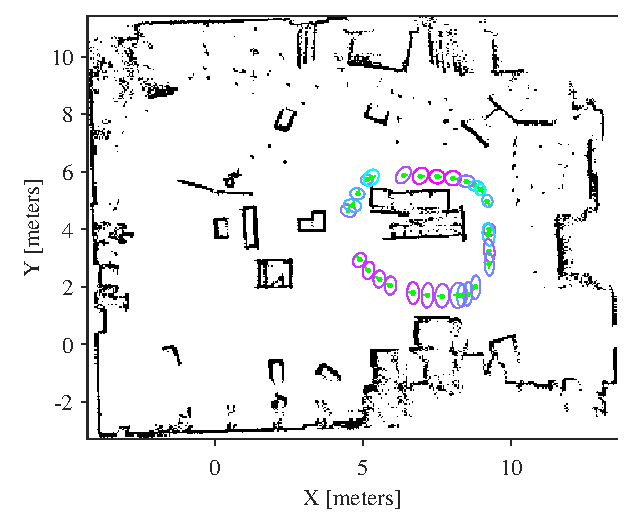
\includegraphics[scale=1.0]{chapters/evaluation/figures/flexlab_path_with_covariance_with_initial_box_positions}
        \end{subfigure}
        \begin{subfigure}[t]{0.2\textwidth}
            \centering
            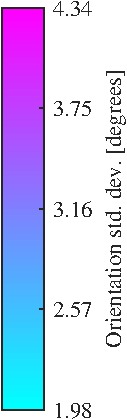
\includegraphics[scale=1.0]{chapters/evaluation/figures/flexlab_path_with_covariance_bar-crop}
        \end{subfigure}
        \caption{Covariances estimated by AMCL, superimposed on the map with boxes in initial position, shown with contours marking one standard deviation around the robot's estimated pose(green).}
        \label{fig:flexlab_path_with_covariance_first_location_map}
\end{figure}

\begin{figure}[htbp]
    \begin{subfigure}[t]{0.7\textwidth}	
        \centering	
        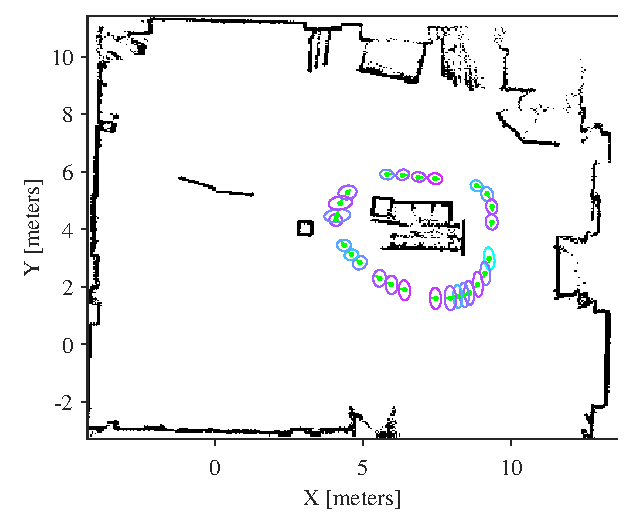
\includegraphics[scale=1.0]{chapters/evaluation/figures/flexlab_path_with_covariance_with_cleaned_map}
    \end{subfigure}
    \begin{subfigure}[t]{0.2\textwidth}
        \centering
        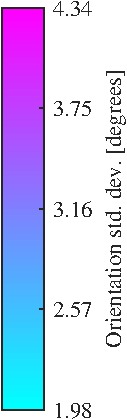
\includegraphics[scale=1.0]{chapters/evaluation/figures/flexlab_path_with_covariance_bar-crop}
    \end{subfigure}
    \caption{Covariances estimated by AMCL, superimposed on the used static map, shown with contours marking one standard deviation around the robot's estimated pose(green).}
    \label{fig:flexlab_path_with_covariance_with_cleaned_map}
\end{figure}

\begin{figure}
\centering
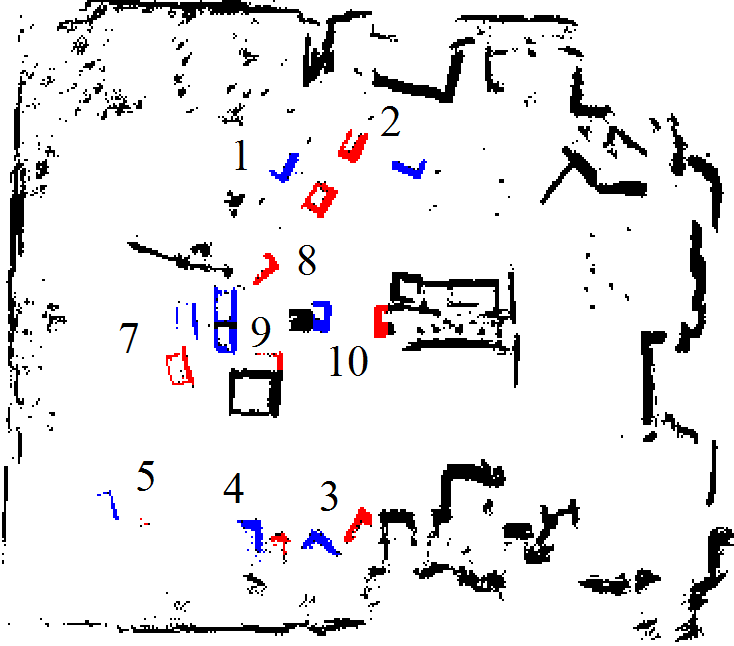
\includegraphics[scale=1.3]{chapters/evaluation/figures/cells_used_for_evaluation_with_identification}
\caption{}
\label{fig:cells_used_for_evaluation_with_identification}
\end{figure}
\begin{figure}
\centering
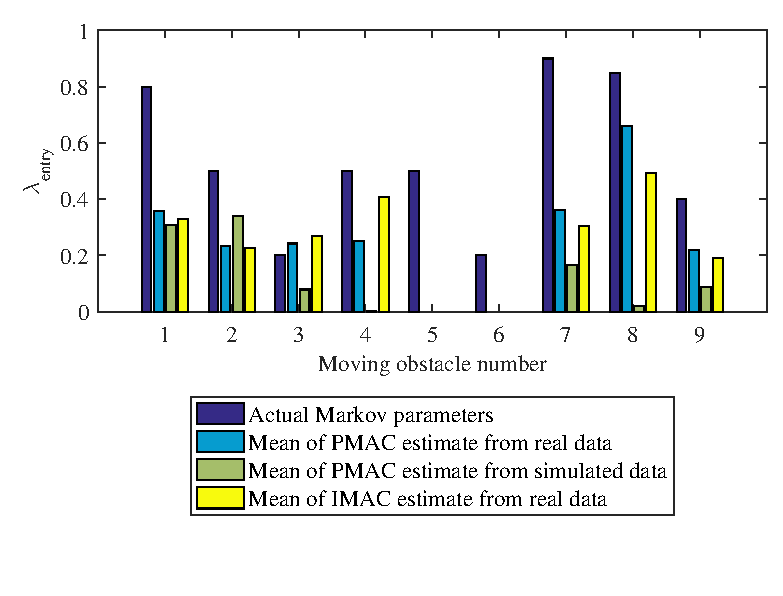
\includegraphics[scale=1]{chapters/evaluation/figures/compare_learned_markov_entry}
\caption{}
\label{fig:compare_learned_markov_entry}
\end{figure}
\begin{figure}
\centering
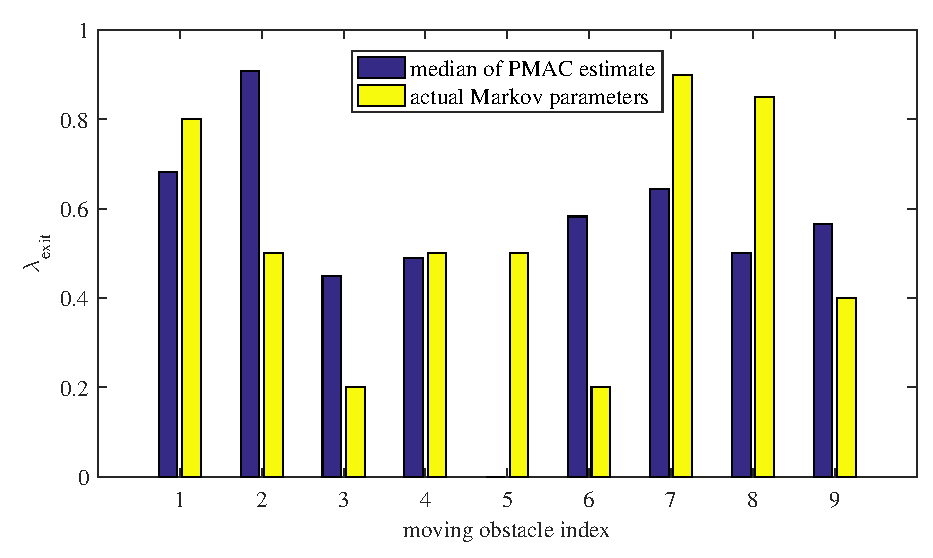
\includegraphics[scale=1]{chapters/evaluation/figures/compare_learned_markov_exit}
\caption{}
\label{fig:compare_learned_markov_exit}
\end{figure}


